\chapter{Viscoplasticity}
\section{VAFCRP Model}
Here we present a versatile viscoplastic model that can be used to model metals under dynamic loadings. It is essentially a multiaxial extension of the aforementioned Armstrong--Fredrick uniaxial model with additional viscosity component. Due to the presence of viscosity, the typical formulation and implementation shall be modified a bit, as now transient effects are accounted for and yield function does not need to be non-positive. It is only used to determine whether a trial state is elastic or plastic.
\subsection{Theory}
\subsubsection{Yield Function}
A von Mises type yielding function is used.
\begin{gather}
f=\sqrt{\dfrac{3}{2}}\norm{\beeta}-k=q-k,
\end{gather}
in which $\beeta=\bs-\bbeta$ is the shifted stress, $\bs$ is the deviatoric stress, $\bbeta$ is the back stress, $k$ is the isotropic hardening stress and $q=\sqrt{\dfrac{3}{2}}\norm{\beeta}$ is the equivalent stress.
\subsubsection{Flow Rule}
The associated plasticity flow is adopted. The plastic strain rate is then
\begin{gather}
\dot{\bvarepsilon^p}=\gamma\pdfrac{f}{\bsigma}=\sqrt{\dfrac{3}{2}}\gamma\bn,
\end{gather}
where $\bn=\dfrac{\beeta}{\norm{\beeta}}$. The corresponding accumulated plastic strain rate is
\begin{gather}
\dot{p}=\sqrt{\dfrac{2}{3}\dot{\bvarepsilon^p}:\dot{\bvarepsilon^p}}=\gamma.
\end{gather}
One shall note that strictly speaking, it shall be the viscous plastic strain rather than the plastic strain. For brevity, the superscript $\left(\cdot\right)^p$ is used. If one wishes, $\left(\cdot\right)^{vp}$ can also be used.
\subsubsection{Plastic Multiplier}
Unlike plasticity, viscoplasticity adopts a different way to determine plastic multiplier. The rate of plastic multiplier is defined as
\begin{gather}
\dfrac{\gamma}{\Delta{}t}=\dfrac{1}{\mu}\left(\left(\dfrac{q}{k}\right)^{\dfrac{1}{\epsilon}}-1\right),
\end{gather}
in which $\Delta{}t$ is increment of pseudo time which shall be available from global time integration method, $\mu$ and $\epsilon$ are two material constants. Here a \cite{Peric1993} type rule is used for easier numerical implementation. Equivalently, after some rearrangement, it is
\begin{gather}
q\left(\dfrac{\Delta{}t}{\Delta{}t+\mu\gamma}\right)^\epsilon-k=0.
\end{gather}
\subsubsection{Hardening Law}
Similar to the previous model, a Voce type exponential function with a linear component is used for isotropic hardening stress.
\begin{gather}
k=\sigma_y+k_lp+k_s-k_se^{-mp}.
\end{gather}
In which, $m$ is a parameter controls the speed of hardening.

The incremental form of multiplicative back stress \cite{Chaboche1989} $\displaystyle\bbeta=\sum\bbeta^i$ is defined as
\begin{gather*}
\dot{\bbeta^i}=\sqrt{\dfrac{2}{3}}a^i\dot{\bvarepsilon^p}-b^i\bbeta^i\dot{p}.
\end{gather*}
Again, $a^i$ and $b^i$ are two sets of model parameters. In terms of $\gamma$, it is $\dot{\bbeta^i}=a^i\gamma{}\bn-b^i\gamma\bbeta^i$.
\subsection{Formulation}
In the following derivation, the subscript $\left(\cdot\right)_{n+1}$ is omitted for brevity.
\subsubsection{Elastic Loading/Unloading}
The trial state can be computed as usual.
\begin{gather}\label{eq:vafcrp_t}
\bsigma^\text{trial}=\bsigma_n+\mb{D}:\left(\bvarepsilon_{n+1}-\bvarepsilon_n\right).
\end{gather}
The trial yield function can be then expressed as
\begin{gather}\label{eq:vafcrp_tf}
f^\text{trial}=\sqrt{\dfrac{3}{2}}\norm{\dev{\bsigma^\text{trial}}-\sum\bbeta_n^i}-k_n.
\end{gather}
\subsubsection{Plastic Evolution}
Given that
\begin{gather}\label{eq:vafcrp_beta}
\bbeta^i=\bbeta_n^i+a^i\gamma\bn-b^i\gamma\bbeta^i,\quad\rightarrow\quad
\bbeta^i=\dfrac{\bbeta_n^i+a^i\gamma\bn}{1+b^i\gamma},
\end{gather}
the shifted stress can be computed as
\begin{gather}
\begin{split}
\beeta&=\bs-\bbeta=2G\mathbb{I}^\text{dev}:\left(\bvarepsilon_{n+1}-\bvarepsilon^p_n-\sqrt{\dfrac{3}{2}}\gamma\bn\right)-\bbeta\\&=\bs^\text{trial}-\sqrt{6}G\gamma\bn-\sum\dfrac{\bbeta_n^i+a^i\gamma\bn}{1+b^i\gamma}
\end{split}
\end{gather}
with $\bs^\text{trial}=2G\mathbb{I}^\text{dev}\left(\bvarepsilon_{n+1}-\bvarepsilon^p_n\right)$. Hence,
\begin{gather*}
\norm{\beeta}\bn+\sqrt{6}G\gamma\bn+\sum\dfrac{a^i\gamma}{1+b^i\gamma}\bn=\bs^\text{trial}-\sum\dfrac{\bbeta_n^i}{1+b^i\gamma},
\end{gather*}
it is easy to see that
\begin{gather}
\left(\norm{\beeta}+\sqrt{6}G\gamma+\sum\dfrac{a^i\gamma}{1+b^i\gamma}\right)\bn=\bs^\text{trial}-\sum\dfrac{\bbeta_n^i}{1+b^i\gamma},
\end{gather}
meaning $\bn$ and $\bs^\text{trial}-\sum\dfrac{\bbeta_n^i}{1+b^i\gamma}$ are coaxial, thus
\begin{gather}
\bn=\dfrac{\beeta}{\norm{\beeta}}=\dfrac{\bs^\text{trial}-\sum\dfrac{\bbeta_n^i}{1+b^i\gamma}}{\norm{\bs^\text{trial}-\sum\dfrac{\bbeta_n^i}{1+b^i\gamma}}}.
\end{gather}
Now both $\beeta$ and $\bn$ shall be functions of $\gamma$, which allows simplification of local system. Based on this fact,
\begin{gather}
\beeta=\norm{\beeta}\bn=\left(\norm{\bs^\text{trial}-\sum\dfrac{\bbeta_n^i}{1+b^i\gamma}}-\sqrt{6}G\gamma-\sum\dfrac{a^i\gamma}{1+b^i\gamma}\right)\bn.
\end{gather}
Furthermore, $q=\sqrt{\dfrac{3}{2}}\left(\norm{\bs^\text{trial}-\sum\dfrac{\bbeta_n^i}{1+b^i\gamma}}-\sqrt{6}G\gamma-\sum\dfrac{a^i\gamma}{1+b^i\gamma}\right)$. Its derivative with regard to $\gamma$ is
\begin{gather}
\pdfrac{q}{\gamma}=\sqrt{\dfrac{3}{2}}\sum\dfrac{b^i\bn:\bbeta_n^i-a^i}{(1+b^i\gamma)^2}-3G.
\end{gather}
\subsubsection{Local Scalar Residual}
For viscoplasticity, the yield function $f$ is not necessarily zero. The rate form of plastic multiplier is used here as the residual.
\begin{gather*}\label{eq:vafcrp_r}
R=q\left(\dfrac{\Delta{}t}{\Delta{}t+\mu\gamma}\right)^\epsilon-k.
\end{gather*}
The corresponding derivatives are then
\begin{gather}\label{eq:vafcrp_dr}
\pdfrac{R}{\gamma}=\left(\dfrac{\Delta{}t}{\Delta{}t+\mu\gamma}\right)^\epsilon\left(\pdfrac{q}{\gamma}-\dfrac{q\epsilon\mu}{\Delta{}t+\mu\gamma}\right)-\ddfrac{k}{\gamma}
\end{gather}
and
\begin{gather}
\pdfrac{R}{\bvarepsilon_{n+1}}=\left(\dfrac{\Delta{}t}{\Delta{}t+\mu\gamma}\right)^\epsilon\sqrt{6}G\bn:\mathbb{I}^\text{dev}=\left(\dfrac{\Delta{}t}{\Delta{}t+\mu\gamma}\right)^\epsilon\sqrt{6}G\bn,
\end{gather}
with
\begin{gather}
\ddfrac{k}{\gamma}=k_l+k_sme^{-m\left(p_n+\gamma\right)}.
\end{gather}
\subsubsection{Consistent Tangent Stiffness}
For stiffness, $\bvarepsilon_{n+1}$ is now varying, then
\begin{gather}
\pdfrac{R}{\bvarepsilon_{n+1}}+\pdfrac{R}{\gamma}\pdfrac{\gamma}{\bvarepsilon_{n+1}}=0,\qquad\pdfrac{\gamma}{\bvarepsilon_{n+1}}=-\left(\pdfrac{R}{\gamma}\right)^{-1}\pdfrac{R}{\bvarepsilon_{n+1}}.
\end{gather}
The stress is
\begin{gather}
\bsigma_{n+1}=\bsigma^\text{trial}-\sqrt{6}G\gamma\bn.
\end{gather}
The derivative is
\begin{gather}\label{eq:vafcrp_stiffness}
\begin{split}
\pdfrac{\bsigma_{n+1}}{\bvarepsilon_{n+1}}&=\mb{D}-\sqrt{6}G\left(\gamma\pdfrac{\bn}{\bvarepsilon_{n+1}}+\left(\bn+\gamma\pdfrac{\bn}{\gamma}\right)\pdfrac{\gamma}{\bvarepsilon_{n+1}}\right)\\
&=\mb{D}+\sqrt{6}G\left(\left(\bn+\gamma\pdfrac{\bn}{\gamma}\right)\left(\pdfrac{R}{\gamma}\right)^{-1}\pdfrac{R}{\bvarepsilon_{n+1}}-\gamma\pdfrac{\bn}{\bvarepsilon_{n+1}}\right).
\end{split}
\end{gather}
In which,
\begin{gather}
\pdfrac{\bn}{\gamma}=\dfrac{\sum\dfrac{b^i}{(1+b^i\gamma)^2}\left(\bbeta_n^i-\left(\bn:\bbeta_n^i\right)\bn\right)}{\norm{\bs^\text{trial}-\sum\dfrac{\bbeta_n^i}{1+b^i\gamma}}},\qquad
\pdfrac{\bn}{\bvarepsilon_{n+1}}=\dfrac{2G\left(\mathbb{I}^\text{dev}-\bn\otimes\bn\right)}{\norm{\bs^\text{trial}-\sum\dfrac{\bbeta_n^i}{1+b^i\gamma}}}.
\end{gather}
\subsection{Implementation}
The state determination algorithm of this VAFCRP model is given in \algoref{algo:vafcrp_model}.
\begin{breakablealgorithm}
\caption{state determination of VAFCRP model}\label{algo:vafcrp_model}
\begin{algorithmic}
\State \textbf{Parameter}: $\lambda$, $G$, $u$, $\epsilon$, $m$, $k_l$, $k_s$, $\sigma_y$, $a^i$, $b^i$
\State \textbf{Input}: $\bvarepsilon_{n+1}$, $\bvarepsilon_n$, $\bsigma_n$, $\bbeta_n^i$, $p_n$, $\Delta{}t$
\State \textbf{Output}: $\mb{D}_{n+1}$, $\bsigma_{n+1}$, $\bbeta_{n+1}^i$, $p_{n+1}$
\State compute $\bsigma^\text{trial}$, $\bs^\text{trial}$, $\bn$ and $f^\text{trial}$\Comment{\eqsref{eq:vafcrp_t} and \eqsref{eq:vafcrp_tf}}
\If {$f^\text{trial}\geqslant0$}
\State $\gamma=0$
\State compute $\bs^\text{trial}$
\While{true}
\State compute $\bn$
\State compute $R$ and $\pdfrac{R}{\gamma}$\Comment{\eqsref{eq:vafcrp_r} and \eqsref{eq:vafcrp_dr}}
\State $\Delta\gamma=\left(\pdfrac{R}{\gamma}\right)^{-1}R$
\If {$\abs{\Delta\gamma}<\text{tolerance}$}
\State break
\EndIf
\State $\gamma\leftarrow\gamma-\Delta\gamma$
\State $p_{n+1}=p_n+\gamma$
\EndWhile
\State $\bsigma_{n+1}=\bsigma^\text{trial}-\sqrt{6}G\gamma\bn$
\State compute all $\bbeta_{n+1}^i$\Comment{\eqsref{eq:vafcrp_beta}}
\State compute $\mb{D}_{n+1}$\Comment{\eqsref{eq:vafcrp_stiffness}}
\Else
\State $\bsigma_{n+1}=\bsigma^\text{trial}$
\State $\bbeta^p_{n+1}=\bbeta^p_n$
\State $p_{n+1}=p_n$
\State $\mb{D}_{n+1}=\mb{D}$
\EndIf
\end{algorithmic}
\end{breakablealgorithm}
\begin{cppcode}
VAFCRP::update_trial_status
\end{cppcode}
\section{Maxwell Model}
The above viscoplasticity models often requires the explicit reference to time $t$ (and its increment $\Delta{}t$). By knowing strain increment $\Delta{}\bvarepsilon$ and $\Delta{}t$, strain rate can be computed by using, for example, constant rate assumption. By such, the whole model can be converted to a form that only depends on strain input, assuming (pseudo-)time is always accessible to local material points. Even with a static analysis setup, creep can be modelled.

Here we present a general framework \cite{Chang2022a} to solve the viscoplasticity model that truly responsive to both strain and strain rate inputs.
\subsection{Background}
For viscous dampers, the mechanical response is often defined in displacement/force. Without loss of generality, a typical viscosity model often defines a linear relationship between stress (force/resistance) $\sigma$ and strain rate (velocity) $\dot{\varepsilon}$,
\begin{gather}
\sigma=\eta\cdot\dot{\varepsilon},
\end{gather}
where $\eta$ is a non-zero constant that is known as the viscosity. Such a linear relationship is known as Newtonian viscosity. For non-Newtonian behaviour, often the power-law fluid is assumed for simplicity \cite{Wu2016}, that is,
\begin{gather}
\sigma=\eta\cdot\sign{\dot{\varepsilon}}\cdot\left\lvert\dot{\varepsilon}\right\rvert^{\alpha},
\end{gather}
where $\alpha$ is a positive constant often known as the flow behaviour index which shall be determined by experiments. If $\alpha=1.0$, the Newtonian viscosity is recovered. A value greater than \num{1.0} represents shear thickening behaviour. For structural dampers, often shear thinning fluid is used, typical values of $\alpha$ range from \num{0.3} to \num{1.0} \cite{Lee2001}. For recent applications, this exponent can be as small as \num{0.1} \cite{Lago2018}.
\subsection{Modified Power-law Viscosity}
Viscous dampers can show different behaviour in four quadrants of strain versus strain rate space. Such a change of behaviour may stem from, for example, applying one-way valves, varying chamber geometries \cite{Hazaveh2017}, changing material types \cite{Lu2018} and/or effective fluid velocity. A constant damping coefficient (viscosity) is not capable of describing such a behaviour (of the device). Instead, it should be defined as a positive function of current state to account for various mechanisms, which is
\begin{gather}
\eta=f\left(\varepsilon,\dot\varepsilon\right)>0.
\end{gather}
Thus the stress can be written as
\begin{gather}\label{eq:quadrant_damper_govern}
\sigma=\eta\left(\varepsilon,\dot\varepsilon\right)\cdot\sign{\dot{\varepsilon}}\cdot\left\lvert\dot{\varepsilon}\right\rvert^{\alpha}.
\end{gather}
It shall be noted that \eqsref{eq:quadrant_damper_govern} can also be expressed as
\begin{gather}
\sigma=\tilde{\eta}\cdot\dot{\varepsilon}
\end{gather}
with $\tilde{\eta}=\eta\left(\varepsilon,\dot\varepsilon\right)\cdot\left\lvert\dot{\varepsilon}\right\rvert^{\alpha-1}$ known as \textit{apparent viscosity}, so that such a modification can still be categorised as the generalised Newtonian fluid model.
%If $\eta$ is strictly defined as a material constant, other equivalent forms may also be applied, one example would be $\sigma=\eta\cdot\sign{\dot{\varepsilon}}\cdot\left\lvert\zeta\left(\varepsilon,\dot\varepsilon\right)\cdot\dot{\varepsilon}\right\rvert^{\alpha}$ where $\zeta\left(\varepsilon,\dot\varepsilon\right)$ is a positive multiplier. In this work, we focus on \eqsref{eq:quadrant_damper_govern}.
The definition of $\eta\left(\varepsilon,\dot\varepsilon\right)$ can be quite flexible in order to describe the desired response. Such a modification mimics semi-active control schemes in which stress feedback can be adjusted based on different strain and strain rates as inputs. For more complex (semi-)active schemes, it can be further defined as a function of other quantities, such as system energy and its history. Two examples are shown as follows to illustrate this feature.
\subsubsection{Proposed Quadrant Modification}\label{sec:quadrant_damper}
The simplest case would be using four different constants for four quadrants of the $\varepsilon$-$\dot{\varepsilon}$ space.
\begin{gather}\label{eq:quadrant_damper}
\eta\left(\varepsilon,\dot\varepsilon\right)=\left\{\begin{array}{lc}
\eta_1,&\varepsilon>0,~\dot{\varepsilon}>0,\\
\eta_2,&\varepsilon<0,~\dot{\varepsilon}>0,\\
\eta_3,&\varepsilon<0,~\dot{\varepsilon}<0,\\
\eta_4,&\varepsilon>0,~\dot{\varepsilon}<0.
\end{array}\right.
\end{gather}

Although \eqsref{eq:quadrant_damper} possesses a simple form that could be easily understood, sudden changes of damping coefficient, as observed on two axes, are practically unrealistic. The rate of transition from one quadrant to another also plays a vital role and affects the overall response. Furthermore, discontinuities in damping coefficient may cause numerical difficulties. Ideally, a smooth transition is required to improve both numerical stability and robustness of the model. To this end, a sigmoid function can be applied. The following arctangent functions provide controllable smooth transition between two sides of the $\dot{\varepsilon}$-axis.
\begin{gather}
\eta_{12}\left(\varepsilon\right)=\dfrac{\eta_1+\eta_2}{2}+\dfrac{\eta_1-\eta_2}{\pi}\arctan\left(g_1\varepsilon\right),\\
\eta_{43}\left(\varepsilon\right)=\dfrac{\eta_4+\eta_3}{2}+\dfrac{\eta_4-\eta_3}{\pi}\arctan\left(g_1\varepsilon\right),
\end{gather}
where $g_1$ is a constant that controls the steepness of the transition region. In a similar fashion, for the $\varepsilon$-axis, the following function can be defined,
\begin{gather}
\eta\left(\varepsilon,\dot\varepsilon\right)=\dfrac{\eta_{12}\left(\varepsilon\right)+\eta_{43}\left(\varepsilon\right)}{2}+\dfrac{\eta_{12}\left(\varepsilon\right)-\eta_{43}\left(\varepsilon\right)}{\pi}\arctan\left(g_2\dot\varepsilon\right),
\end{gather}
where $g_2$ is another constant that serves a similar purpose to that of $g_1$. The damping coefficient $\eta$ can now be expressed as a function of four material constants, viz.,
\begin{multline}\label{eq:arctan_transition}
\eta\left(\varepsilon,\dot\varepsilon\right)=\dfrac{\eta_1+\eta_2+\eta_3+\eta_4}{4}+\dfrac{\eta_1-\eta_2+\eta_3-\eta_4}{\pi^2}\arctan\left(g_1\varepsilon\right)\arctan\left(g_2\dot\varepsilon\right)\\+\dfrac{\eta_1-\eta_2-\eta_3+\eta_4}{2\pi}\arctan\left(g_1\varepsilon\right)+\dfrac{\eta_1+\eta_2-\eta_3-\eta_4}{2\pi}\arctan\left(g_2\dot\varepsilon\right).
\end{multline}

Noting that a sudden change of damping response is not achievable in real life, constants $g_1$ and $g_2$ (strictly speaking, only the one corresponds to displacement tolerance, viz., $g_1$) can hence represent physical manufacturing tolerance of pistons and chambers.

Apart from the arctangent function, other types of sigmoid curves can also be used. The following is an alternative using the logistic function.
\begin{gather}
\eta\left(\varepsilon,\dot\varepsilon\right)=\eta_3+\dfrac{\eta_4-\eta_3}{1+e^{-g_1\varepsilon}}+\dfrac{\eta_2-\eta_3}{1+e^{-g_2\dot{\varepsilon}}}+\dfrac{\eta_1+\eta_3-\eta_2-\eta_4}{\left(1+e^{-g_1\varepsilon}\right)\left(1+e^{-g_2\dot{\varepsilon}}\right)}.
\end{gather}
It shall be noted that the derivatives of \eqsref{eq:arctan_transition} have a simpler form than that of the above definition. Other simple functions such as a linear function can also be applied, in which the transition range can be explicitly defined.

The quadrant modification can be customised to mimic the effect of negative-stiffness damping \cite{Iemura2009,Hoegsberg2011,Zhou2015,Javanbakht2018} by choosing large $\eta_2$ and $\eta_4$ and small $\eta_1$ and $\eta_3$. Further elaborations are shown in numerical examples. Readers who are interested in practical applications of such a quadrant damper can refer to, for example, the work by \cite{Hazaveh2017}.
\subsection{Extension to Maxwell Model}
In some certain applications, dampers could be idealised as Maxwell models given the fact that the extender braces are not fully rigid \cite{Makris1991}. For classic viscoelasticity and viscoplasticity, theories have been developed \cite{Simo1998}. Simple cases can be solved analytically by using convolution integrals. Consider a typical Maxwell model, the rheology model is often represented by \figref{fig:rheology_maxwell}.
\begin{figure}[ht]
\centering\scriptsize
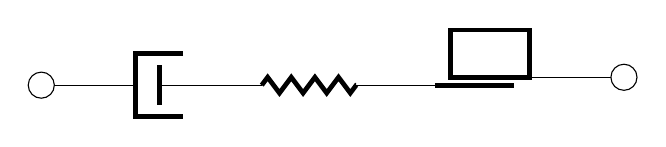
\begin{tikzpicture}[scale=2]
\draw(1.8,0)node[circle,draw,fill=white]{}--(2.4,0)(2.55,0)--(3.2,0)(3.8,0)--++(.6,0)(4.9,.05)--++(.6,0)node[circle,draw,fill=white]{};
\draw[line width=.6mm](2.7,.2)--++(-.3,0)--++(0,-.4)--++(.3,0)(2.55,.125)--++(0,-.25)(4.3,0)--++(.5,0)(4.4,.05)rectangle(4.9,.35);
\draw[line width=.6mm,decorate,decoration={zigzag,segment length=3mm, amplitude=1mm}](3.2,0)--++(.6,0);
\end{tikzpicture}
\caption{rheology model of the Maxwell model with inelastic spring}\label{fig:rheology_maxwell}
\end{figure}
It is normally represented by two components in series: a viscous dashpot and a rate-independent spring which can be either elastic (without frictional device) or elasto-plastic (with frictional device), then the total strain $\varepsilon$ and stress $\sigma$ of the model can be expressed as
\begin{gather}\label{eq:equal_strain}
\varepsilon=\varepsilon_d+\varepsilon_s,\\\label{eq:equal_stress}
\sigma=\sigma_d=\sigma_s.
\end{gather}
For a generalised case, it is also possible to further write stress feedback as functions of the corresponding strain and strain rate, which is
\begin{gather}
\sigma_d=f(\varepsilon_d,\dot\varepsilon_d),\qquad\sigma_s=g(\varepsilon_s).
\end{gather}
The subscripts $\cdot_d$ and $\cdot_s$ represent dashpot and spring part, respectively. By differentiating total strain with respect to time, one could obtain
\begin{gather}\label{eq:equal_strain_rate}
\dot\varepsilon=\dot\varepsilon_d+\dot\varepsilon_s.
\end{gather}
The governing equation can be established via \eqsref{eq:equal_stress} so that
\begin{gather}\label{eq:governing_equation}
\sigma_d-\sigma_s=0.
\end{gather}
\subsection{Formulation}
In terms of numerical simulation, using a dashpot alone does not require special treatments since the corresponding damping force can be treated as external load and directly applied to the system/structure/model. If needed, the damping modulus can be derived accordingly. This also applies to the case if the damper is idealised as a Kelvin--Voigt model. However, for a Maxwell model, due to the presence of coupling between dashpot and spring, a proper algorithm is required for state determinations of both components. Some researchers use the popular Bouc-Wen \cite{Wen1976} model to simulate viscous dampers \cite{Gong2016,Chang2016}. However, the identification and calibration of model parameters often impose unnecessary complexities to the model. Alternatively, the Maxwell system can be solved by using ODE solvers. In this section, the drawbacks of the ODE solver based approach are first discussed, followed by the proposition of a new iterative algorithm with better accuracy and efficiency.
\subsubsection{ODE Solver Based Approach}\label{sec:ode_issue}
If a linear elastic spring and a constant $\eta$ are adopted, the whole system can be converted into an ordinary differential equation via \eqsref{eq:equal_strain_rate}, that is,
\begin{gather}
\dot\varepsilon=\dot\varepsilon_d+\dot\varepsilon_s=\sign{\sigma}\sqrt[\alpha]{\dfrac{\left\vert\sigma\right\vert}{\eta}}+\dfrac{\dot\sigma}{E},
\end{gather}
where $E$ denotes the elastic modulus of the spring element, so that
\begin{gather}\label{eq:maxwell_ode}
\dot\sigma=E\left(\dot\varepsilon-\sign{\sigma}\sqrt[\alpha]{\dfrac{\left\vert\sigma\right\vert}{\eta}}\right).
\end{gather}
By assuming a proper distribution of total strain rate $\dot\varepsilon$ over time $t$, viz., $\dot\varepsilon=\dot\varepsilon(t)$, \eqsref{eq:maxwell_ode} can be written as a function of $\sigma$ and $t$, viz., $\dot\sigma=f(\sigma,t)$. Sophisticated solvers for ordinary differential equations, including explicit, implicit and semi-implicit solvers, can be applied to solve this system. Such an approach has been used in prior research \cite{Kasai2004,Akcelyan2018}. For some simple cases, analytical solutions can also be derived \cite{Hatada2000}.

Although the above method is simple, straightforward and easy to implement, it suffers from three main drawbacks.
\begin{enumerate}
\item
Applicability. Such an approach cannot be applied to inelastic spring. For which, unless the corresponding spring constitutive model is \textbf{stress driven}, which is not the case for most constitutive models, spring strain (rate) cannot be recovered from total stress (rate) since it depends on loading history. As a consequence, dashpot strain (rate) cannot be recovered. Because of this reason, the damping coefficient $\eta$ can only be a function of total strain and total strain rate (instead of that of dashpot), however, dashpot response solely depends on its own strain and strain rate according to the definition. This is \textbf{theoretically incorrect}. As can be seen later, the discrepancy due to different strain and strain rate measures adopted can sometimes be significant, depending on the specific parameter set used.

Even with elastic spring, either linear or nonlinear, since spring strain is not explicitly included in \eqsref{eq:maxwell_ode}, there is no consistent way to isolate spring/dashpot strain (rate) from total strain (rate) without interpolating both total strain and total strain rate. This then leads to the second issue.
\item
Kinematics Compatibility. This problem stems from the assumed distribution of total strain rate $\dot\varepsilon$, which should be carefully defined by taking the global level time integration method into account. On one hand, the global time integration scheme is often not known to local material points. Analysts may switch from one global time integration method to another, resulting in different integrations of total strain at local points. On the other hand, an arbitrarily defined distribution of $\dot\varepsilon$, such as a simple linear relationship \cite{Akcelyan2018}, would lead to a corresponding strain increment which is independent from the one computed by the global time integration. A consistency/compatibility issue arises. This is less concerning if the time step is sufficiently small.
\item
Efficiency. Existing ODE solvers are less efficient in terms of solving such a Maxwell model. Consider the classic Fehlberg method \cite{Fehlberg1969} as an example, by construction, it requires six evaluations of \eqsref{eq:maxwell_ode} for every new $\sigma$. If the error of the current step is unacceptable, all previously evaluated function values would be discarded and a smaller step size needs to be chosen to repeat the whole computation procedure. Sub-iterations may be further required to meet a small tolerance.

Besides, if a shear thinning power-law fluid is used, when $\alpha$ deviates from unity ($\alpha<1$), \eqsref{eq:maxwell_ode} tends to be stiff when velocity (strain rate) is close to zero and results in potential numerical instability. In that case, explicit methods fail and lower order implicit solvers have to be used, and the computational cost skyrockets due to their low order of convergence (second order at most due to the second Dahlquist barrier \cite{Dahlquist1963}). Similar stability issues may also occur if spring stiffness is disproportionally too large.

Furthermore, since the only independent variable is time $t$, it is in general difficult to derive the tangent moduli for global equation solving, resulting in a superlinear global convergence rate at most.
\end{enumerate}
More accurate results can be achieved with fewer function evaluations and thus less computation time if a better solving method is available. The ideal algorithm shall strictly comply with the theory and possess a higher convergence rate. Moreover, there is still room for improvements of both applicability and efficiency/robustness.
\subsubsection{Proposed Iterative Approach}
Here a typical strain driven framework is assumed. For numerical simulation, at a single material point, it is generally difficult to obtain the exact relationship between total strain $\varepsilon$ and total strain rate $\dot\varepsilon$ as they are determined by the global integration algorithm that could be changed on demand. To ensure kinematic compatibility, similar to the strategy adopted in many time integration methods, the following assumption can be made between two adjacent steps $t^n$ and $t^{n+1}=t^n+\Delta{}t$ with $\chi=\varepsilon$ denoting the total strain of the Maxwell model and $\dot\chi=\dot\varepsilon$ denoting its strain rate,
\begin{gather}
\chi^{n+1}=\chi^n+\left(\left(1-\beta\right)\dot\chi^n+\beta\dot\chi^{n+1}\right)\Delta{}t,
\end{gather}
or equivalently with $\Delta\chi=\chi^{n+1}-\chi^n$ and $\Delta\dot\chi=\dot\chi^{n+1}-\dot\chi^n$ denoting increments of $\chi$ and its rate,
\begin{gather}\label{eq:newmark2}
\Delta\chi=\left(\dot\chi^n+\beta\Delta\dot\chi\right)\Delta{}t,
\end{gather}
where $\beta$ is an integration parameter. For $\beta=0.5$, a constant acceleration rule is implied. Since there is no other constraint imposed, such an integration relationship can be alternatively applied to either spring component ($\chi=\varepsilon_s$) or dashpot component ($\chi=\varepsilon_d$). By such a manner, kinematic compatibility can be rigorously satisfied within the Maxwell model and is independent from the global time integration method. The parameter $\beta$ can be defined as a user input (if $\chi=\varepsilon_s$ or $\chi=\varepsilon_d$) or be solved internally (if $\chi=\varepsilon$), which is
\begin{gather}\label{eq:delta}
\beta=\dfrac{\Delta\varepsilon-\dot\varepsilon^n\Delta{}t}{\Delta\dot\varepsilon\Delta{}t},
\end{gather}
by using total strains $\varepsilon^{n+1}$ and $\varepsilon^n$ and total strain rates $\dot\varepsilon^n$ and $\dot\varepsilon^{n+1}$, since they are given at the beginning of each time step at a specific material point.

As aforementioned, the damping coefficient can be defined as a function of dashpot strain $\varepsilon_d$ and dashpot strain rate $\dot\varepsilon_d$, it is necessary to compute them explicitly as history variables. Here an iterative method is presented to solve for all strain and strain rate components.

With the above basic formulae at hand, the problem can now be rephrased as: knowing $\varepsilon^n$, $\dot\varepsilon^n$, $\varepsilon^n_d$, $\dot\varepsilon^n_d$, $\varepsilon^n_s$ and $\dot\varepsilon^n_s$, given the total increments $\Delta\varepsilon=\varepsilon^{n+1}-\varepsilon^n$ and $\Delta\dot\varepsilon=\dot\varepsilon^{n+1}-\dot\varepsilon^n$, find increments $\Delta\varepsilon_d$, $\Delta\varepsilon_s$, $\Delta\dot\varepsilon_d$ and $\Delta\dot\varepsilon_s$ that satisfy
\begin{gather}
\label{eq:condense_a}\Delta\varepsilon_d+\Delta\varepsilon_s=\Delta\varepsilon,\\
\label{eq:condense_b}\Delta\dot\varepsilon_d+\Delta\dot\varepsilon_s=\Delta\dot\varepsilon,\\
\label{eq:condense_c}\Delta\varepsilon_s-\beta\Delta\dot\varepsilon_s\Delta{}t=\dot\varepsilon^n_s\Delta{}t,\\
\label{eq:condense_d}\sigma_d(\varepsilon^{n+1}_d,\dot\varepsilon^{n+1}_d)-\sigma_s(\varepsilon^{n+1}_s)=0.
\end{gather}
It shall be pointed out that \eqsref{eq:condense_c} is the implementation of \eqsref{eq:newmark2} on spring strain $\varepsilon_s$. In this case, the parameter $\beta$ can be either computed from \eqsref{eq:delta} or given as a model constant. \eqsref{eq:newmark2} can also be applied on dashpot strain $\varepsilon_d$. However, additional conversions between different quantities may be required.

Since $\dot\varepsilon_s$ does not enter the constitutive relationship of spring, it can be condensed out so that \eqsref{eq:condense_b} and \eqsref{eq:condense_c} can be combined to
\begin{gather}\label{eq:condense_e}
\Delta\varepsilon_s+\beta\Delta\dot\varepsilon_d\Delta{}t=\dot\varepsilon^n_s\Delta{}t+\beta\Delta\dot\varepsilon\Delta{}t.
\end{gather}

\eqsref{eq:condense_a}, \eqsref{eq:condense_d} and \eqsref{eq:condense_e} can be iteratively solved with the classic Newton-Raphson method. Alternatively, other optimisers can be applied. Linearisation of these equations leads to the Jacobian matrix $\mb{J}$ and the corresponding residual $\mb{R}$ for increment $\mathbf{x}=\begin{bmatrix}\delta\varepsilon_s&\delta\varepsilon_d&\delta\dot\varepsilon_d\end{bmatrix}^\mT$, which are
\begin{gather}
\mb{J}=-\begin{bmatrix}
	1                                          & 1                               & 0                                   \\[2mm]
	1                                          & 0                               & \beta\Delta{}t                      \\[2mm]
	-\dfrac{\md{\sigma_s}}{\md{\varepsilon_s}} & \pdfrac{\sigma_d}{\varepsilon_d} & \pdfrac{\sigma_d}{\dot\varepsilon_d}
\end{bmatrix},\qquad
\mb{R}=\begin{bmatrix}
	\Delta\varepsilon-\Delta\varepsilon_s^k-\Delta\varepsilon_d^k                                                                  \\
	\dot\varepsilon^n_s\Delta{}t+\beta\Delta\dot\varepsilon\Delta{}t-\Delta\varepsilon_s^k-\beta\Delta\dot\varepsilon_d^k\Delta{}t \\
	\sigma^k_s-\sigma^k_d
\end{bmatrix},
\end{gather}
where the superscript $\left(\cdot\right)^k$ denotes the $k$-th local iteration.

The determinant of $\mb{J}$ reads
\begin{gather}
\det{\mb{J}}=\beta\Delta{}t\left(\dfrac{\md{\sigma_s}}{\md{\varepsilon_s}}+\pdfrac{\sigma_d}{\varepsilon_d}\right)+\pdfrac{\sigma_d}{\dot\varepsilon_d}.
\end{gather}
Clearly in the current setup, there is no guarantee for $\mb{J}$ to be strictly invertible. If $\mb{J}$ appears to be ill-conditioned, low rank updates such as the BFGS method, which do not rely on Jacobian, can be used to solve the system. The inverse $\mb{J}^{-1}$ can be analytically expressed as
\begin{gather}\label{eq:inv_j}
\mb{J}^{-1}=\dfrac{-1}{\det{\mb{J}}}\begin{bmatrix}
	\pdfrac{\sigma_d}{\varepsilon_d}\beta\Delta{}t                                               & \pdfrac{\sigma_d}{\dot\varepsilon_d}                                       & -\beta\Delta{}t \\[3mm]
	\dfrac{\md{\sigma_s}}{\md{\varepsilon_s}}\beta\Delta{}t+\pdfrac{\sigma_d}{\dot\varepsilon_d} & -\pdfrac{\sigma_d}{\dot\varepsilon_d}                                      & \beta\Delta{}t  \\[3mm]
	-\pdfrac{\sigma_d}{\varepsilon_d}                                                            & \dfrac{\md{\sigma_s}}{\md{\varepsilon_s}}+\pdfrac{\sigma_d}{\varepsilon_d} & 1
\end{bmatrix}.
\end{gather}
\eqsref{eq:inv_j} can be directly used in iterations. The computation of the numerical inverse of the Jacobian can be avoided so that the rounding error in float point arithmetic can be minimised as long as $\det{\mb{J}}$ is not zero.
\subsubsection{A Simple Case}
In the case of nonlinear spring and constant damping coefficient $\eta$,
\begin{gather}
\dfrac{\md{\sigma_s}}{\md{\varepsilon_s}}=E(\varepsilon_s),\qquad\pdfrac{\sigma_d}{\varepsilon_d}=0,\qquad\pdfrac{\sigma_d}{\dot\varepsilon_d}=\eta\alpha\left\lvert\dot\varepsilon_d\right\rvert^{\alpha-1}.
\end{gather}

Given that $\beta>0$, $\eta>0$, $\alpha>0$ and $\Delta{}t>0$, for the determinant to be strictly positive,
\begin{gather}
E(\varepsilon_s)>-\dfrac{\eta\alpha}{\beta\Delta{}t}\left\lvert\dot\varepsilon_d\right\rvert^{\alpha-1}.
\end{gather}
Thus a non-softening spring would lead to a nonsingular Jacobian. For softening response, viz., $E(\varepsilon_s)<0$,
\begin{gather}
\dot\varepsilon_d\neq\pm\sqrt[\alpha-1]{\dfrac{\beta\Delta{}t{}\left\lvert{}E(\varepsilon_s)\right\rvert}{\eta\alpha}}
\end{gather}
guarantees an invertible Jacobian.

Furthermore, if the spring is linear elastic and $\alpha=1$, the Jacobian is constant so all quantities can be solved in one step. To solve such a system with the aforementioned ODE solver based approach, multiple function evaluations are inevitable, although the analytical solution is available.
\subsubsection{Tangent Stiffness and Damping Moduli}
For an easier derivation of tangent stiffness and damping moduli, the stress response can be rewritten as follows,
\begin{gather}
\sigma=\dfrac{1}{2}\left(\sigma_s+\sigma_d\right).
\end{gather}
Since $\sigma_s=\sigma_d$, in fact, any weighted average with non-zero weights can be used. At equilibrium, the residual equals zero vector, viz., $\mb{R}=\mb{0}$, differentiation results in
\begin{gather}
\pdfrac{\mb{R}}{\mb{a}}\md{\mb{a}}+\pdfrac{\mb{R}}{\mb{x}}\md{\mb{x}}=\mb{0},
\end{gather}
in which $\mb{a}=\begin{bmatrix}
\Delta\varepsilon&\Delta\dot\varepsilon
\end{bmatrix}^\mT$ is the increments of total strain and total strain rate and $\pdfrac{\mb{R}}{\mb{x}}=\mb{J}$. Thus,
\begin{gather}\label{eq:internal}
\pdfrac{\mb{x}}{\mb{a}}=\begin{bmatrix}\pdfrac{\mb{x}}{\Delta\varepsilon}&\pdfrac{\mb{x}}{\Delta\dot\varepsilon}\end{bmatrix}=-\mb{J}^{-1}\pdfrac{\mb{R}}{\mb{a}}=\dfrac{1}{\det{\mb{J}}}\begin{bmatrix}
	\pdfrac{\sigma_d}{\varepsilon_d}\beta\Delta{}t                                               & \pdfrac{\sigma_d}{\dot\varepsilon_d}\beta\Delta{}t                                                     \\[3mm]
	\dfrac{\md{\sigma_s}}{\md{\varepsilon_s}}\beta\Delta{}t+\pdfrac{\sigma_d}{\dot\varepsilon_d} & -\pdfrac{\sigma_d}{\dot\varepsilon_d}\beta\Delta{}t                                                    \\[3mm]
	-\pdfrac{\sigma_d}{\varepsilon_d}                                                            & \dfrac{\md{\sigma_s}}{\md{\varepsilon_s}}\beta\Delta{}t+\pdfrac{\sigma_d}{\varepsilon_d}\beta\Delta{}t
\end{bmatrix}.
\end{gather}
It shall be pointed out that the parameter $\beta$ is assumed to be a constant user input in the above derivation for brevity. If it is expressed as a function of $\mb{a}$ via \eqsref{eq:delta}, the corresponding $\partial\mb{x}/\partial\mb{a}$ can be derived accordingly. The procedure is presented in the appendix. The stiffness and damping moduli can be readily computed by using the chain rule. Knowing that
\begin{gather}\label{eq:moduli}
\pdfrac{\sigma}{\mb{x}}=\dfrac{1}{2}\begin{bmatrix}
\ddfrac{\sigma_s}{\varepsilon_s}&\pdfrac{\sigma_d}{\varepsilon_d}&\pdfrac{\sigma_d}{\dot\varepsilon_d}
\end{bmatrix},
\end{gather}
then after some rearrangements,
\begin{gather}\label{eq:tangent}
K=\pdfrac{\sigma}{\varepsilon}=\dfrac{\beta\Delta{}t}{\det{\mb{J}}}\ddfrac{\sigma_s}{\varepsilon_s}\pdfrac{\sigma_d}{\varepsilon_d},\qquad{}C=\pdfrac{\sigma}{\dot\varepsilon}=\dfrac{\beta\Delta{}t}{\det{\mb{J}}}\ddfrac{\sigma_s}{\varepsilon_s}\pdfrac{\sigma_d}{\dot\varepsilon_d}.
\end{gather}
\eqsref{eq:tangent} is independent from the global time integration scheme and quadratic convergence is recovered. It can be easily verified that if the dashpot behaves like a spring so that $\md{\sigma_s}/\md{\varepsilon_s}=K_1$, $\md{\sigma_d}/\md{\varepsilon_d}=K_2$ and $\md{\sigma_d}/\md{\dot\varepsilon_d}=0$, then the stiffness modulus $K$ falls back to the widely recognised form of two springs in series,
\begin{gather}
K=\dfrac{K_1K_2}{K_1+K_2}.
\end{gather}
\subsubsection{Circumventions of Potential Numerical Difficulties}
Numerical difficulties may arise if $\partial\eta/\partial\varepsilon_d$ becomes too large due to an improperly large steepness parameter $g_1$. The same situation occurs with $\partial\eta/\partial\dot\varepsilon_d$ and $g_2$. This problem can be eased by scaling steepness parameters according to the maximum strain and strain rate. Another major problem is that $\partial\sigma_d/\partial\dot\varepsilon_d$ approaches infinity at origin if the exponent $\alpha$ in power-law model is smaller than unity. An enough-close-to-origin strain rate can be often met, especially in forced vibrations. This may not be a problem if the corresponding damping modulus term $\partial\sigma_d/\partial\dot\varepsilon_d$ is not involved in the global equation of motion, in which case the quadratic convergence rate cannot be recovered. However, when combined with a spring to form a Maxwell model, an disproportionally large $\partial\sigma_d/\partial\dot\varepsilon_d$ may fail the local iteration. A possible workaround would be limiting the apparent viscosity to a finite value via extrapolation \cite{Wu1998}.

Here in lieu of the original power-law relationship, a cubic segment within a small width around origin is used to limit the corresponding derivative within a finite value so that the stress feedback can be rewritten as a piecewise-defined function such as
\begin{gather}
\sigma_d=\left\{
\begin{array}{ll}
\eta\left(\varepsilon_d,\dot\varepsilon_d\right)\cdot\left(A\dot{\varepsilon}_d^3+B\dot{\varepsilon}_d\right),&\left\lvert\dot{\varepsilon}_d\right\rvert\leqslant{}v,\\
\eta\left(\varepsilon_d,\dot\varepsilon_d\right)\cdot\sign{\dot{\varepsilon}_d}\cdot\left\lvert\dot{\varepsilon}_d\right\rvert^{\alpha},&\text{else},
\end{array}
\right.
\end{gather}
where $v$ is a user-defined constant that controls the size of cubic replacement. The cubic function, as an odd function, is chosen given the fact that the power-law \eqsref{eq:quadrant_damper_govern} is also an odd function. With a cubic replacement, $C^1$ continuity can be ensured. By enforcing continuity of both $\sigma_d$ and $\partial\sigma_d/\partial\dot\varepsilon_d$ at $\left\lvert\dot{\varepsilon}_d\right\rvert=v$, constants $A$ and $B$ can be solved as
\begin{gather}
A=\dfrac{\alpha-1}{2}v^{\alpha-3},\qquad
B=\dfrac{3-\alpha}{2}v^{\alpha-1}.
\end{gather}
Hence,
\begin{gather}\label{eq:max_der}
\pdfrac{\sigma_d}{\dot{\varepsilon}_d}\Big\vert_{\dot{\varepsilon}_d=0}=\eta\left(\varepsilon_d,\dot\varepsilon_d\right)\Big\vert_{\dot{\varepsilon}_d=0}B=\eta\left(\varepsilon_d,\dot\varepsilon_d\right)\Big\vert_{\dot{\varepsilon}_d=0}\dfrac{3-\alpha}{2}v^{\alpha-1}.
\end{gather}
A properly defined $v$ can greatly improve the performance of the proposed model for a small $\alpha$ as the apparent viscosity is bounded with such a modification. In the meantime, the damping stress is not largely affected since the strain rate is close to zero.
\subsection{Implementation}
\begin{cppcode}
Maxwell::update_trial_status(const vec& t_strain, const vec& t_strain_rate)
\end{cppcode}